\chapter{Resultados e Discussão}
\label{cap:resultados}

Este capítulo apresenta os resultados da avaliação de desempenho do motor de inferência,
conduzida segundo o protocolo descrito na Seção~\ref{sec:estrategia-testes}. Os resultados
são organizados nos dois regimes de execução previstos, o regime irrestrito e o regime de
seleção parcial, seguidos de uma análise comparativa que relaciona a evidência empírica
obtida às questões de pesquisa formuladas no Capítulo~\ref{cap:01}.

\section{Regime Irrestrito}
\label{sec:resultado-irrestrito}

No regime irrestrito, os domínios de todas as categorias permanecem completos, situação que
corresponde ao catálogo antes de qualquer seleção do usuário. A
Tabela~\ref{tab:bench-regime1} apresenta o desempenho dos dois motores para tamanhos de
domínio crescentes.

\begin{table}[htbp]
  \centering
  \caption{Desempenho dos motores no regime irrestrito}
  \label{tab:bench-regime1}
  \resizebox{\ifdim\width>\linewidth\linewidth\else\width\fi}{!}{%
    \begin{tabular}{rrrrrcr}
      \toprule
      $d$ & AC-3 checagens & AC-3 tempo (ms) & FB checagens         & FB tempo (ms) & FB concl. & Espaço residual       \\
      \midrule
      10  & 118            & 0,093           & 152000               & 5,586         & sim       & 100000                \\
      25  & 302            & 0,039           & $1{,}46\times10^{7}$ & 510,548       & sim       & $9{,}77\times10^{6}$  \\
      50  & 608            & 0,076           & $1{,}50\times10^{8}$ & 5183,057      & não       & $3{,}13\times10^{8}$  \\
      75  & 915            & 0,101           & $1{,}51\times10^{8}$ & 5191,575      & não       & $2{,}37\times10^{9}$  \\
      100 & 1225           & 0,128           & $1{,}50\times10^{8}$ & 5443,806      & não       & $1{,}00\times10^{10}$ \\
      250 & 3058           & 0,288           & $1{,}63\times10^{8}$ & 6014,267      & não       & $9{,}77\times10^{11}$ \\
      500 & 6125           & 0,637           & $2{,}26\times10^{8}$ & 10076,577     & não       & $3{,}13\times10^{13}$ \\
      \bottomrule
    \end{tabular}%
  }
  \fonte{Elaborada pelo autor}
\end{table}

Os dados evidenciam duas observações centrais. A primeira diz respeito à força bruta, cujo
custo cresce em conformidade com a natureza exponencial do produto cartesiano. A avaliação
exaustiva conclui apenas para os menores valores de $d$, atingindo o teto de aborto a partir
de $d=50$, quando o número de combinações a examinar ultrapassa a ordem de $10^8$. A partir
desse ponto, os valores registrados para a força bruta correspondem ao custo acumulado até a
interrupção, e não ao custo total que a avaliação demandaria, o qual cresceria até
$3{,}13\times10^{13}$ combinações em $d=500$.

A segunda observação diz respeito ao AC-3, que conclui em todos os valores de $d$ em tempo
inferior a um milissegundo, executando algumas milhares de avaliações de restrição mesmo no
maior cenário, com $6{,}125$ checagens em $d=500$. Observa-se, contudo, que o espaço residual
produzido pelo AC-3 permanece exatamente igual a $d^5$ em todos os casos, o que indica que a
arco-consistência não removeu nenhum valor dos domínios.

Essa ausência de poda não constitui ineficiência do motor, mas era prevista pela análise estrutural da Subseção 2.4.2. Com domínios completos sobre um grafo acíclico, cada valor de uma variável encontra suporte em ao menos um valor de cada variável vizinha, de modo que a rede já se apresenta arco-consistente e nenhum valor se torna elegível à remoção. O motor executa, verifica a consistência e encerra sem podar. A
Figura~\ref{fig:bench-checagens} ilustra esse contraste, no qual a curva da força bruta
acompanha a progressão teórica de $d^5$ até atingir o teto de aborto, ao passo que a curva do
AC-3 permanece praticamente constante em ordens de magnitude inferiores.

\begin{figure}[htb]
  \centering
  \caption{Número de avaliações de restrição em função do tamanho do domínio $d$}
  \label{fig:bench-checagens}
  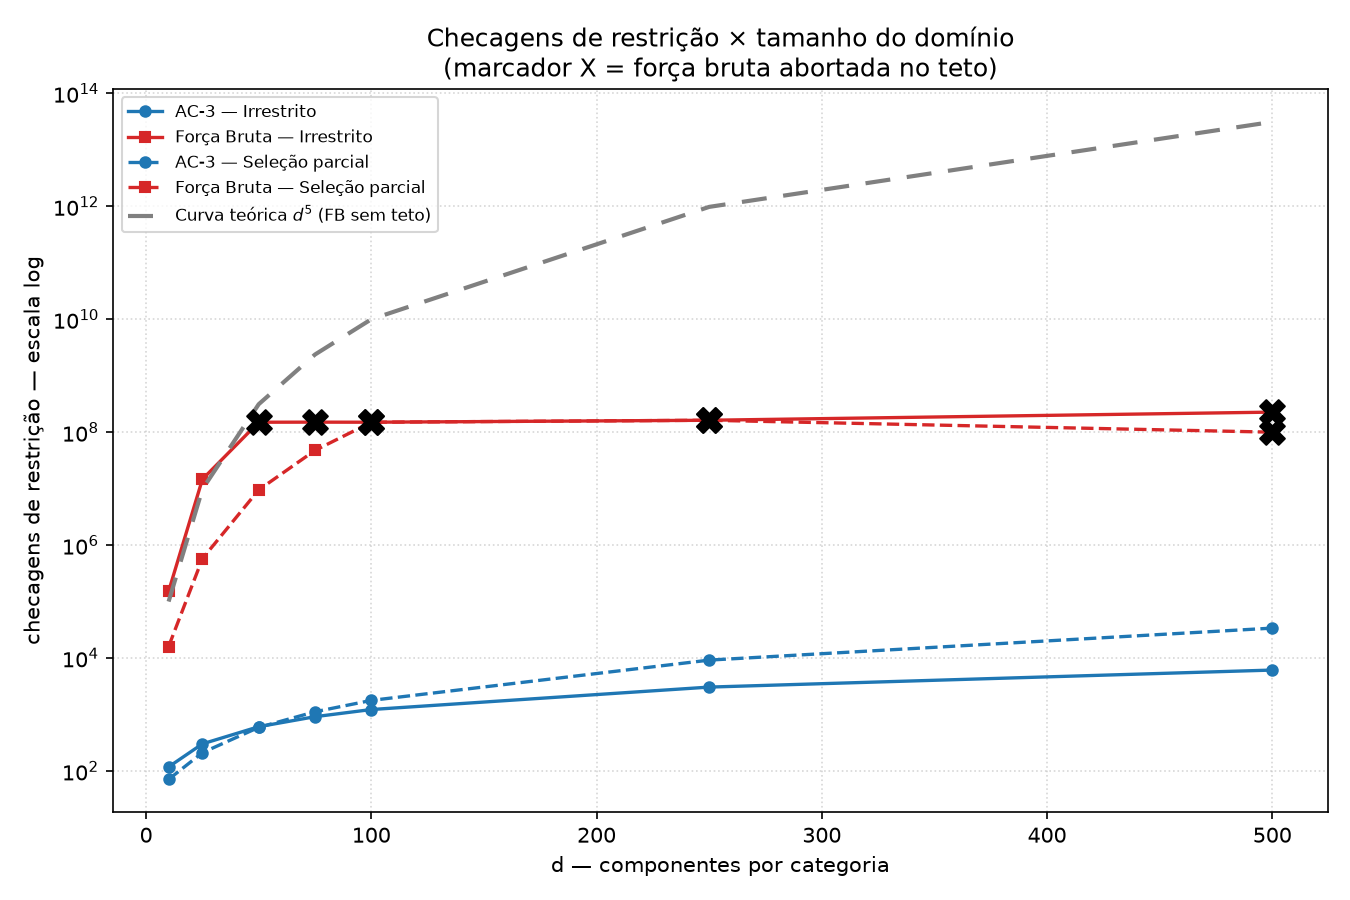
\includegraphics[width=0.85\textwidth]{imagens/output/fig_checagens.png}
  \fonte{Elaborada pelo autor}
\end{figure}

\section{Regime de Seleção Parcial}
\label{sec:resultado-selecao}

No regime de seleção parcial, uma das variáveis é fixada em um único valor, situação que
corresponde a uma etapa intermediária do wizard, na qual o usuário já selecionou um
componente. Para este experimento, fixou-se a categoria CPU em um processador de soquete AM5.
A Tabela~\ref{tab:bench-regime2} apresenta os resultados.

\begin{table}[htbp]
\centering
\caption{Desempenho dos motores no regime de seleção parcial}
\label{tab:bench-regime2}
\resizebox{\ifdim\width>\linewidth\linewidth\else\width\fi}{!}{%
\begin{tabular}{rrrrrcrr}
\toprule
$d$ & AC-3 checagens & AC-3 tempo (ms) & FB checagens & FB tempo (ms) & FB concl. & Residual & Redução ($d^5$/residual) \\
\midrule
10 & 71 & 0,038 & 16000 & 0,558 & sim & 1500 & $\times$67 \\
25 & 211 & 0,030 & 574375 & 21,256 & sim & 45000 & $\times$217 \\
50 & 591 & 0,055 & $9{,}50\times10^{6}$ & 344,182 & sim & 812500 & $\times$385 \\
75 & 1118 & 0,082 & $4{,}76\times10^{7}$ & 1711,388 & sim & $3{,}95\times10^{6}$ & $\times$600 \\
100 & 1778 & 0,217 & $1{,}50\times10^{8}$ & 5433,302 & não & $1{,}25\times10^{7}$ & $\times$800 \\
250 & 9191 & 0,294 & $1{,}63\times10^{8}$ & 6148,752 & não & $4{,}92\times10^{8}$ & $\times$1984 \\
500 & 33878 & 1,222 & $1{,}00\times10^{8}$ & 2830,519 & não & $7{,}81\times10^{9}$ & $\times$4000 \\
\bottomrule
\end{tabular}%
}
\fonte{Elaborada pelo autor}
\end{table}

Diferentemente do regime anterior, a arco-consistência agora produz poda efetiva. Ao fixar a
CPU em um único valor de soquete AM5, todas as placas-mãe de soquete distinto perdem seu
único suporte possível e são removidas do domínio. Essa remoção propaga-se de forma
transitiva à categoria RAM, uma vez que a eliminação das placas de soquete incompatível
elimina também o suporte aos módulos de memória de padrão correspondente. Como consequência,
o espaço residual cai muito abaixo de $d^5$, com uma redução que evolui de $\times67$ em
$d=10$ a $\times4000$ em $d=500$.

A composição do espaço residual explicita o mecanismo da poda. Para $d=50$, o residual de
$812{,}500$ configurações decompõe-se no produto entre a CPU fixada, as $13$ placas-mãe de
soquete AM5 remanescentes, os $25$ módulos de memória de padrão DDR5 remanescentes e as $50$
GPUs e $50$ fontes preservadas. As categorias GPU e Fonte não sofrem poda porque participam
apenas da restrição quantitativa de capacidade energética, não sendo afetadas pela seleção do
soquete da CPU. Esse comportamento reproduz precisamente o de um CSP dinâmico, no qual cada
decisão do usuário restringe o conjunto de valores admissíveis das variáveis relacionadas
\cite{Mittal1989}.

Cabe observar que, neste regime, o AC-3 executa um número maior de avaliações de restrição
que no regime irrestrito, alcançando $33{,}878$ checagens em $d=500$ contra $6{,}125$ no caso
irrestrito. Esse acréscimo decorre da própria propagação, pois cada remoção de valor implica
a reinserção dos arcos afetados na fila para reverificação. O custo adicional é, todavia,
desprezível em termos absolutos, mantendo-se em $1{,}222$ ms, e é largamente compensado pela
redução de ordens de magnitude no espaço de busca resultante.

\section{Análise Comparativa}
\label{sec:resultado-comparativo}

A Tabela~\ref{tab:bench-comparativa} confronta os dois regimes para um mesmo tamanho de
domínio, $d=50$, sintetizando as duas naturezas distintas de ganho observadas.

\begin{table}[htbp]
  \centering
  \caption{Comparação entre os regimes para $d = 50$}
  \label{tab:bench-comparativa}
  \begin{tabular}{lrr}
    \toprule
    Métrica                & Irrestrito           & Seleção parcial      \\
    \midrule
    Espaço residual (AC-3) & $3{,}13\times10^{8}$ & 812500               \\
    $d^5$ (teórico)        & $3{,}13\times10^{8}$ & $3{,}13\times10^{8}$ \\
    AC-3 checagens         & 608                  & 591                  \\
    AC-3 tempo (ms)        & 0,076                & 0,055                \\
    FB checagens           & $1{,}50\times10^{8}$ & $9{,}50\times10^{6}$ \\
    FB concl.              & não                  & sim                  \\
    FB config.\ válidas    & ---                  & 749125               \\
    \bottomrule
  \end{tabular}
  \fonte{Elaborada pelo autor}
\end{table}

A comparação evidencia que o motor de inferência oferece duas economias complementares. No
regime irrestrito, ainda que não haja poda, o AC-3 decide a consistência da rede com $608$
avaliações de restrição, ao passo que a força bruta não conclui a enumeração sequer dentro do
teto estabelecido. Trata-se de um ganho puramente algorítmico, decorrente de o motor não
necessitar percorrer o espaço de configurações completas. No regime de seleção parcial,
soma-se a esse ganho a poda propagada, que reduz o espaço residual de $3{,}13\times10^{8}$
para $812{,}500$ configurações. Nesse cenário, a força bruta passa a concluir a enumeração e
identifica $749{,}125$ configurações válidas, valor coerente com o espaço residual reportado
pelo AC-3, uma vez que este constitui um limite superior sobre o conjunto de soluções.

A Figura~\ref{fig:bench-tempo} apresenta o tempo de execução dos dois motores em ambos os
regimes, corroborando, sob a métrica temporal, o comportamento já observado sob a métrica de
avaliações de restrição.

\begin{figure}[htb]
  \centering
  \caption{Tempo de execução em função do tamanho do domínio $d$, por regime}
  \label{fig:bench-tempo}
  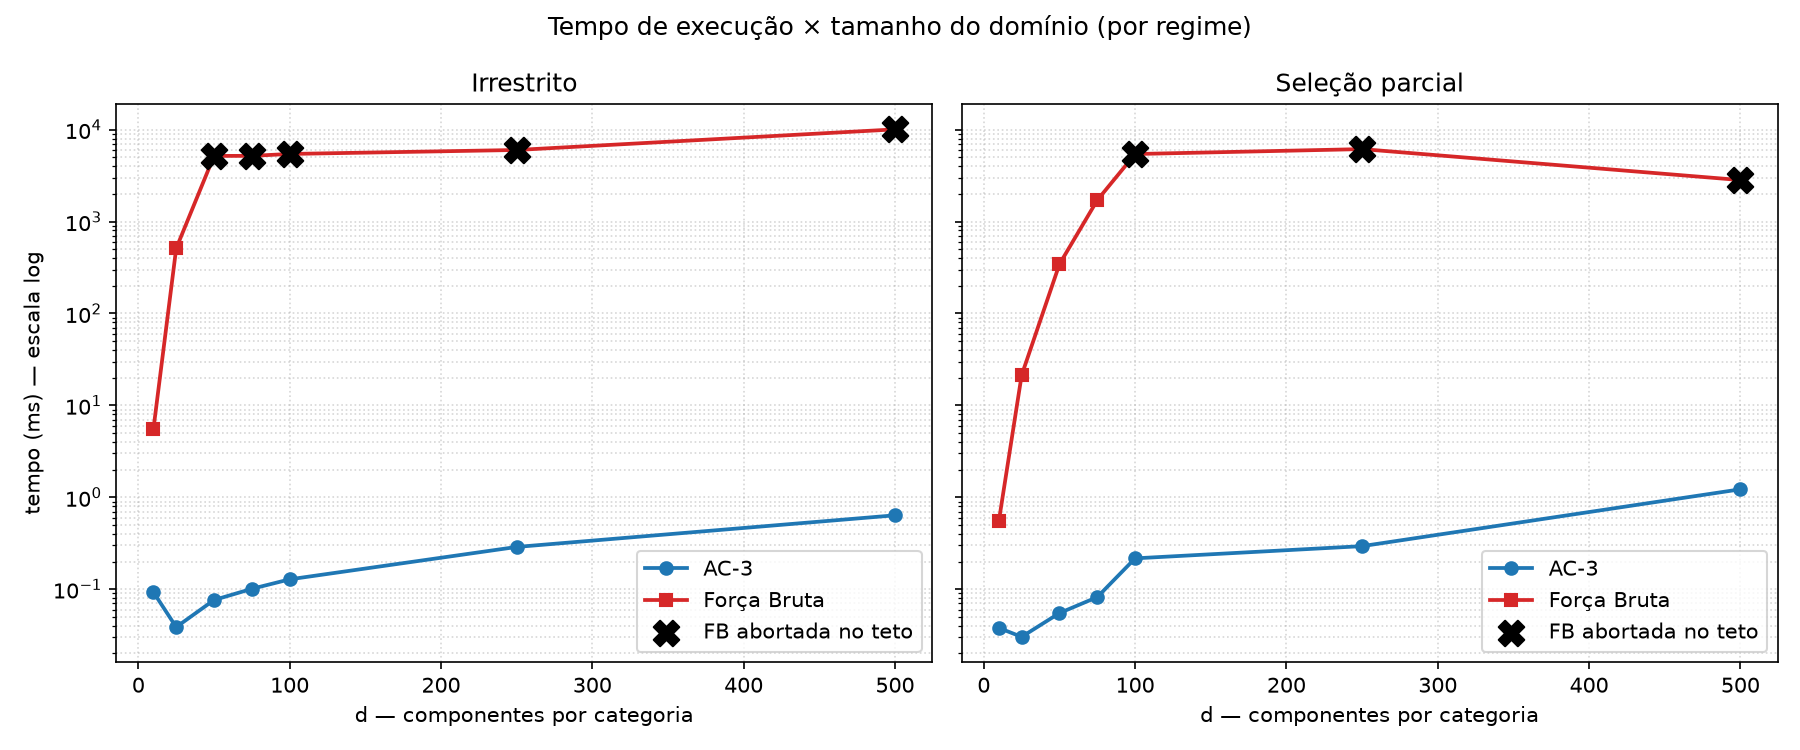
\includegraphics[width=0.85\textwidth]{imagens/output/fig_tempo.png}
  \fonte{Elaborada pelo autor}
\end{figure}

Os resultados sustentam empiricamente a resposta à questão de pesquisa de natureza técnica
formulada no Capítulo~\ref{cap:01}. A validação de configurações de hardware por meio de
propagação de restrições mostra-se viável em tempo praticamente constante e em ordens de
magnitude inferiores à avaliação exaustiva, cuja inviabilidade, decorrente da natureza
NP-completa do CSP, é confirmada pela impossibilidade de conclusão da força bruta a partir de
$d=50$. Confirma-se, ainda, que o efeito de redução de domínio característico da propagação de
restrições manifesta-se precisamente sob seleção parcial, situação que corresponde ao uso real
do sistema, no qual o usuário constrói sua configuração de forma incremental.